%
% 4fAufbau.tex -- Bild zum Thema Optische Fourier-Transformation <opt>
%
% (c) 2023 Marco Niederberger, Yanick Schoch; OST Ostschweizer Fachhochschule
%

\documentclass[tikz]{standalone}
\usepackage{times}
\usepackage{txfonts}
\usepackage{pgfplots}

\pgfplotsset{compat=1.16}
\def\skala{1}

\usetikzlibrary{arrows,intersections,math}
\usetikzlibrary{decorations.markings, calc}

%
% opt_common.tex -- Commands and color definition for the paper <opt>
%
% (c) 2023 Marco Niederberger, Yanick Schoch; OST Ostschweizer Fachhochschule
%

%%% NEW COMMANDS %%%

% Lense (x, height, curvature)
\newcommand{\lense}[3]{
    \def\curvature{0.2}
    \path[fill=glass, draw=black, line width = 0.6, opacity=0.8] (#1,-#2) .. controls (#1 - #3,0) .. (#1,#2) .. controls (#1 + #3,0) .. (#1,-#2);
}

% Dimension arrow (xStart, xEnd, yHeight, text)
\newcommand{\optMeasurement}[4]{%
    \draw[<->] (#1, #3)--(#2, #3) node[above,midway] {#4};
}

% Annotated point
\newcommand{\point}[3]{
    \draw[fill=black] (#1) circle (1pt) node[#3] {#2};
}

%%% COLORS %%%

% Define Color
\definecolor{glass}{cmyk}{0.2,0,0,0}
\colorlet{optBlue}{blue!70!black}
\colorlet{optRed}{red!90!black}

%%% STYLES %%%

% Laser rays
\tikzset{red ray/.style = {optRed, line width = 0.6}}
\tikzset{ray arrow/.style = {red ray, postaction=decorate,decoration={markings,mark=at position 0.52 with \arrow{stealth}}}}


%% Axis (x, textAbove, textBelow)
\newcommand{\xAxis}[3]{%
    \def\lenseX{2.1}
    \draw[->, thin] (#1,-\lenseX)--(#1,\lenseX) node[above]{#2};
    \node[] at (#1, -\lenseX - 0.5){#3};
}

\begin{document}

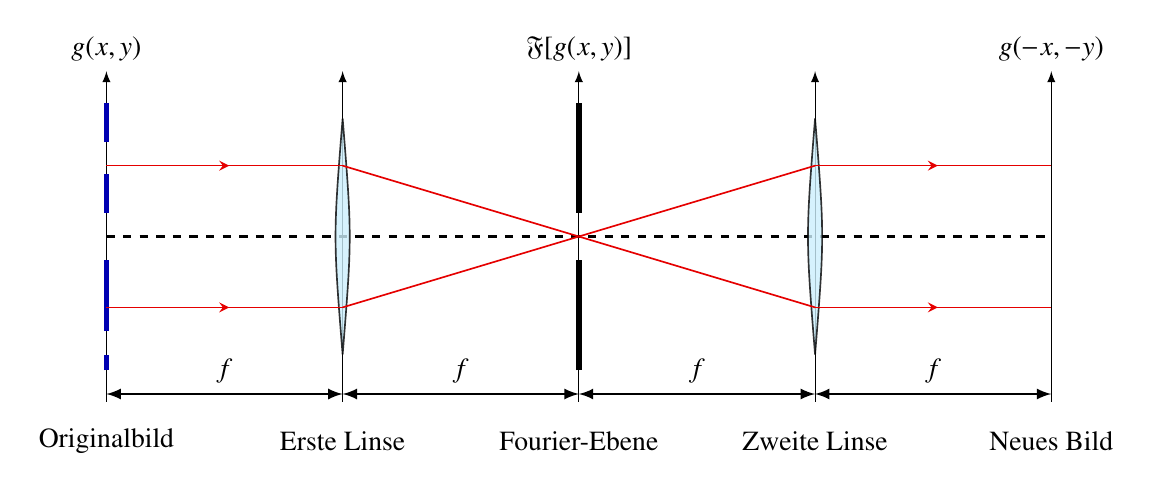
\begin{tikzpicture}[>=latex,thick,scale=\skala]

    % Force the boundary to be symmetric around (0,0)
    \draw[draw=none](-7,0)--(7,0);

    % xAxis
    \xAxis{-6}{$g(x,y)$}{Originalbild}
    \xAxis{-3}{}{Erste Linse}
    \xAxis{0}{$\mathfrak{F}[g(x,y)]$}{Fourier-Ebene}
    \xAxis{3}{}{Zweite Linse}
    \xAxis{6}{$g(-x,-y)$}{Neues Bild}

    % Optical plane
    \draw[dashed] (-6,0)--(6,0);

    % Dimension between the lenses
    \foreach \n in {-2,...,1}{
        \optMeasurement{\n * 3}{\n * 3 + 3}{-2}{$f$}
    }

    % Lenses
    \lense{-3}{1.5}{.12}
    \lense{3}{1.5}{.12}

    % Aperture
    \draw[-, line width=2, optBlue] (-6,-1.7)--(-6,-1.5);
    \draw[-, line width=2, optBlue] (-6,-1.2)--(-6,-0.3);
    \draw[-, line width=2, optBlue] (-6,0.3)--(-6,0.8);
    \draw[-, line width=2, optBlue] (-6,1.2)--(-6,1.7);

    % Laser wave
    % \draw[red ray] (-6.1, -2.1)--(-6.1,2.1);
    % \draw[red ray] (-6.5, -2.1)--(-6.5,2.1) node[above,midway, sloped, inner sep = 2] {\small{Gerade Wellenfront}};
    % \draw[red ray] (-6.9, -2.1)--(-6.9,2.1);
    % \optMeasurement{-6.5}{-6.1}{-2}{$\lambda$}

    % Low pass filter
    \draw[-, line width=2, black] (0,-1.7)--(0,-0.3);
    \draw[-, line width=2, black] (0,0.3)--(0,1.7);

    % Rays
    \draw[ray arrow] (-6,0.9) -- (-3,0.9);
    \draw[red ray] (-3,0.9) -- (3,-0.9);
    \draw[ray arrow] (3,-0.9) -- (6,-0.9);

    \draw[ray arrow] (-6,-0.9) -- (-3,-0.9);
    \draw[red ray] (-3,-0.9) -- (3,0.9);
    \draw[ray arrow] (3,0.9) -- (6,0.9);

\end{tikzpicture}
\end{document}

